%This is a template file for use of iopjournal.cls

\documentclass{iopjournal}
\bibliographystyle{IEEEtran}
\usepackage{float}
\usepackage{amsmath}
\usepackage{tikz}
\usepackage{fix-cm} % Allow scalable Computer Modern fonts to avoid font substitution warnings
\usepackage{listings}

% Options
%  [anonymous]  Provides output without author names, affiliations or acknowledgments to facilitate double-anonymous peer-review
%
% The following packages are required by iopjournal.cls and do not need to be declared again:
%  graphicx
%  fancyhdr
%  xcolor
%  hyperref
%

\begin{document}

\articletype{Tarea 7} %	 e.g. Paper, Letter, Topical Review...

\title{Aplicación de Kernel con Convolución}

\author{Daniel González$^1$\orcid{0000--0000--0000--0000}}

\affil{$^1$Facultad de Ingeniería, Universidad Autónoma de Querétaro, Querétaro, México \\ 14/10/2025}

\email{dgonzalez16@alumnos.uaq.mx}

\keywords{Python, kernel, convolución, preprocesamiento, imagenes, filtros}

\begin{abstract}
En este trabajo se presenta la aplicación de filtros basados en kernels a una imagen utilizando el método de convolución, 
con la libreria OpenCV de Python como de forma manual. Se busca demostrar el funcionamiento de 
la operación de convolución y analizar su efecto sobre la imagen original al modificar los valores del kernel. Mediante la
comparación entre ambos enfoques, se verificó la similiritud en los resultados ademas de demostrar de manera clara como se aplican 
los filtros más alla de solo usar una función la cual nos permite resaltar bordes, suavizar o realzar detalles en imágenes digitales.
\end{abstract}


\section{Introducción}
El reconocimiento de patrones y el procesamiento de imágenes frecuentemente requieren operaciones de filtrado para resaltar características relevantes. La convolución con kernels pequeños (por ejemplo 3×3) es una operación fundamental para detectar bordes, suavizar ruido o realzar detalles. En este reporte se describen los kernels utilizados, la implementación en Python con OpenCV y la implementación manual, y se muestran resultados sobre imágenes de ejemplo.

\section{Materiales y métodos}
\subsection{Kernels empleados}
A continuación se listan los kernels usados en la libreta de Python. Se definen como matrices 3×3:

\begin{lstlisting}[language=Python, caption={Kernels usados (ejemplo)}]
K1 = [[0,0,0],
      [0,1,0],
      [0,0,0]]

K2 = [[ 1, 0,-1],
      [ 0, 1, 0],
      [-1, 0, 1]]

K3 = [[ 0,-1, 0],
      [-1, 4,-1],
      [ 0,-1, 0]]

K4 = [[-1,-1,-1],
      [-1, 8,-1],
      [-1,-1,-1]]

K5 = [[ 0,-1, 0],
      [-1, 5,-1],
      [ 0,-1, 0]]

K6 = (1/16)*[[1,2,1],
             [2,4,2],
             [1,2,1]]
\end{lstlisting}

K3 y K4 son kernels Laplacianos para detección de bordes; K5 es un realce (sharpen) y K6 un suavizado tipo gaussiano.

\section{Desarrollo}
\subsection{Implementación con OpenCV}
OpenCV ofrece la función \texttt{cv2.filter2D (src, ddepth, kernel)} que realiza la convolución de forma sencilla. 
Es importante mencionar que la libreria de OpenCV separa los canales BGR (Blue, Green, Red) diferente al tipico RGB (Red, Green, Blue), 
se aplica \texttt{filter2D} por canal y luego se normaliza el resultado para visualizarlo.

Código:
\begin{figure}[H]
        \centering
        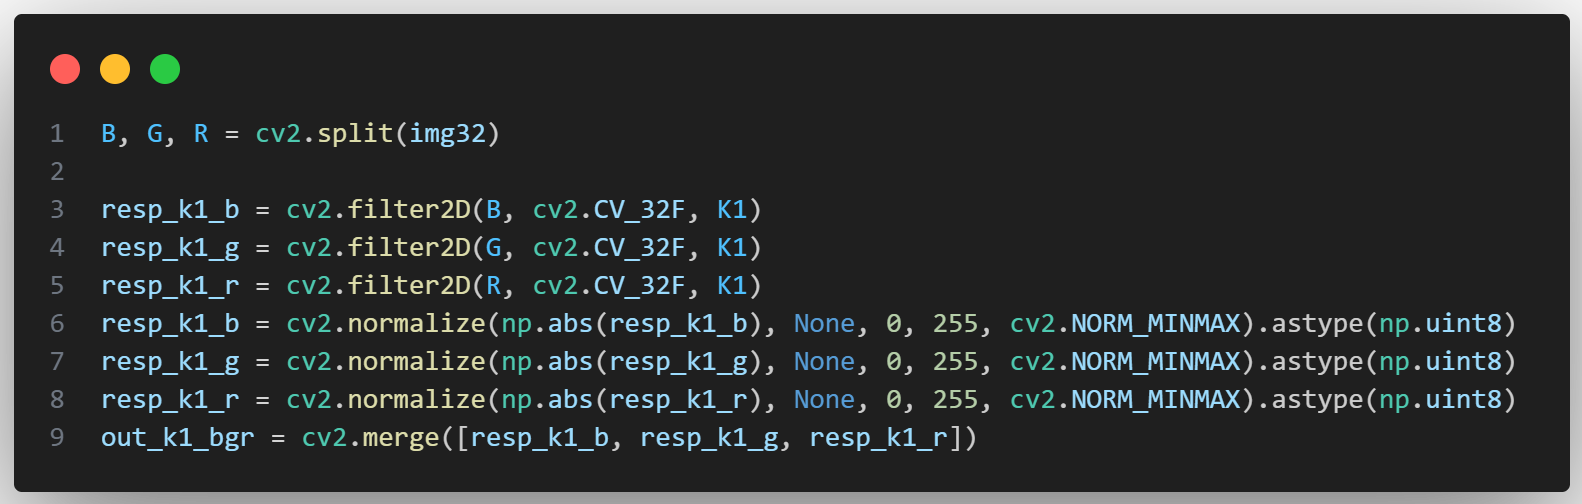
\includegraphics[width=0.8\textwidth]{rsc/opencv.png}
        \caption{Uso de OpenCV para aplicar filtros}
\end{figure}

\subsection{Implementación manual}
La convolución manual consiste en:
\begin{enumerate}
  \item Calcular padding apropiado (reflect o zero).
  \item Para cada píxel (y,x) y cada canal: extraer la vecindad del tamaño del kernel.
  \item Realizar la suma elemento a elemento entre la vecindad y el kernel.
  \item Guardar el valor en la salida; aplicar post-procesado (valor absoluto y normalización para visualizar).
\end{enumerate}

Código:
\begin{figure}[H]
        \centering
        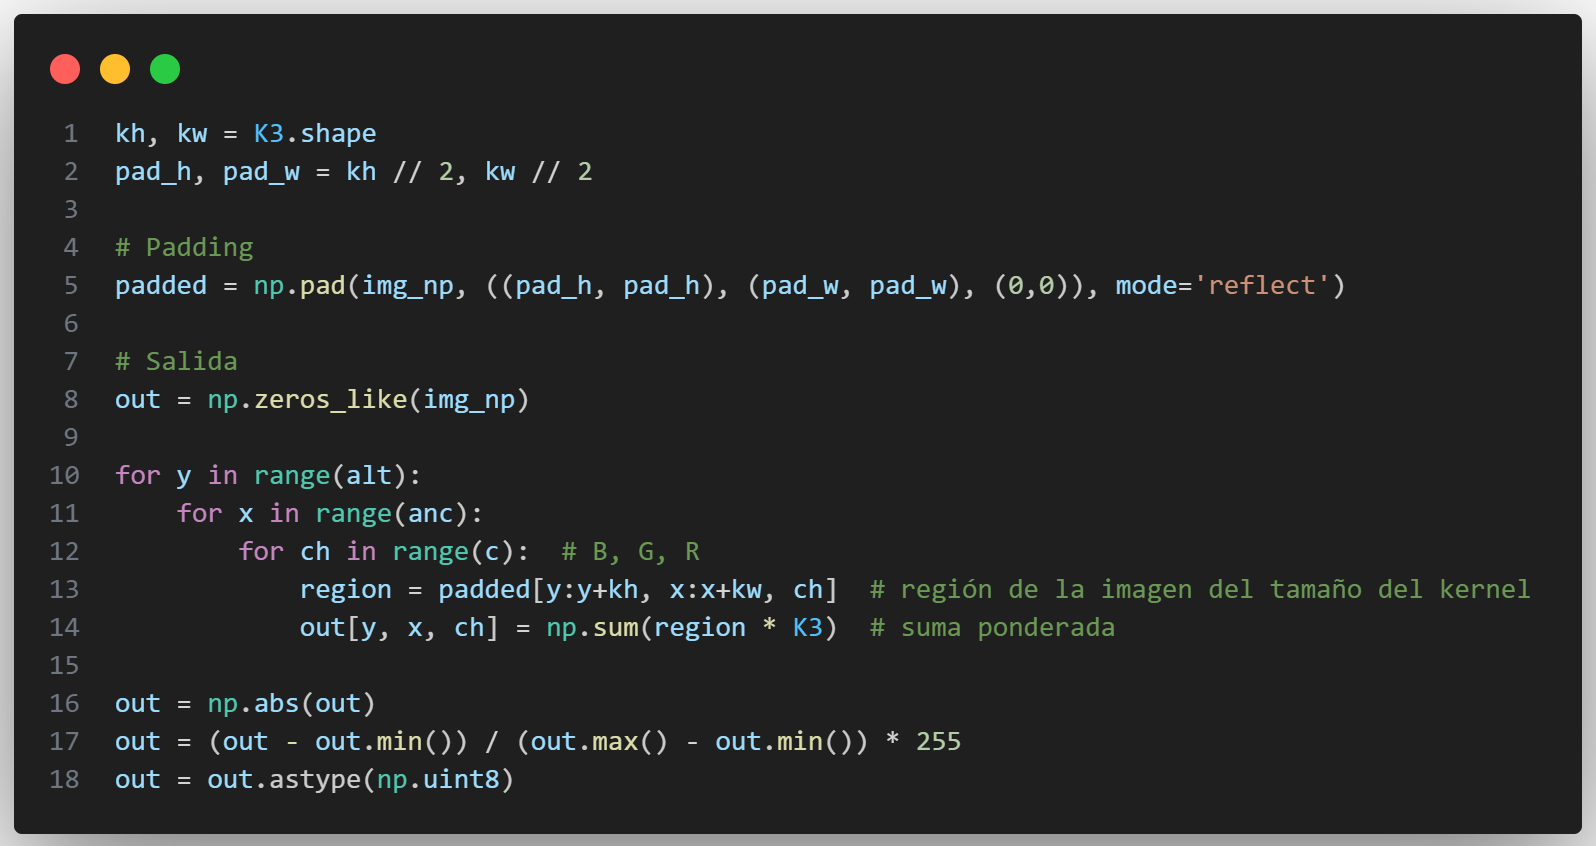
\includegraphics[width=0.8\textwidth]{rsc/manual.png}
        \caption{Implementación manual de convolución}
\end{figure}

\section{Resultados}
\subsection{OpenCV}

\begin{figure}[H]
        \centering
        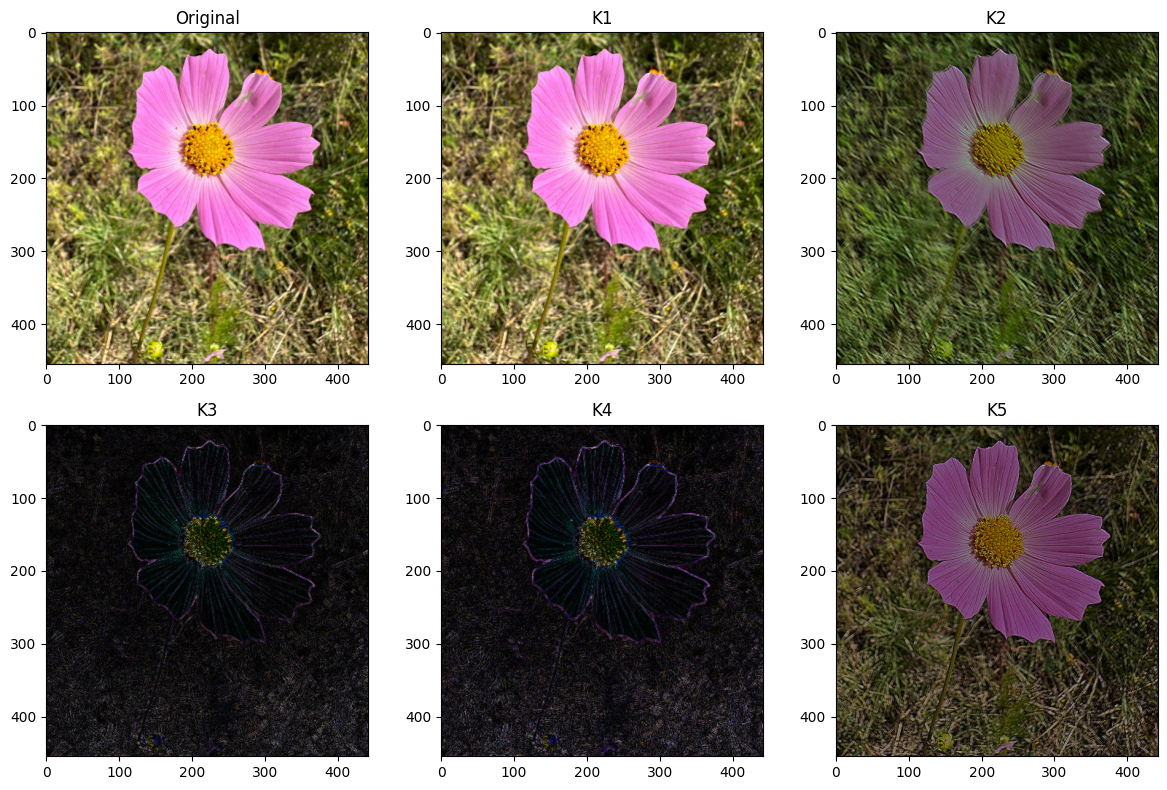
\includegraphics[width=1\textwidth]{rsc/kernel_cv.png}
        \caption{Resultados con OpenCV}
\end{figure}

\subsection{Implementación manual}
\begin{figure}[H]
        \centering
        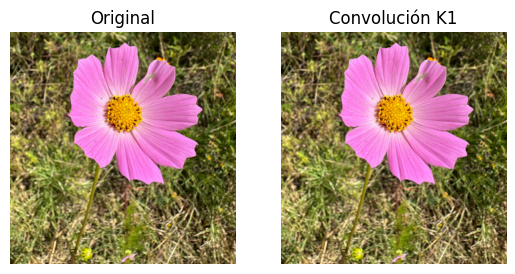
\includegraphics[width=0.7\textwidth]{rsc/k1.png}
        \caption{Resultados con implementación manual (K1)}
\end{figure}
\begin{figure}[H]
        \centering
        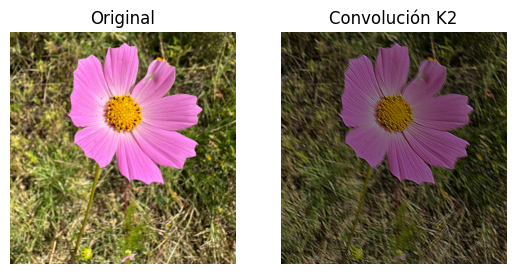
\includegraphics[width=0.7\textwidth]{rsc/k2.png}
        \caption{Resultados con implementación manual (K2)}
\end{figure}
\begin{figure}[H]
        \centering
        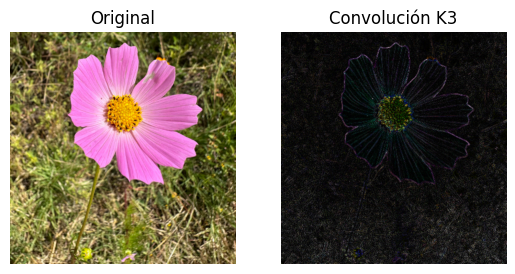
\includegraphics[width=0.7\textwidth]{rsc/k3.png}
        \caption{Resultados con implementación manual (K3)}
\end{figure}
\begin{figure}[H]
        \centering
        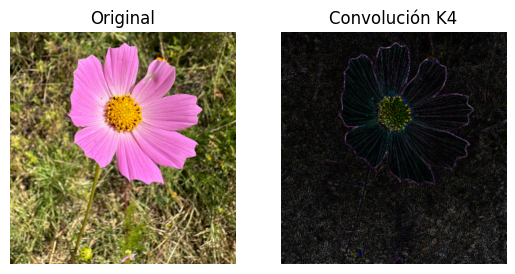
\includegraphics[width=0.7\textwidth]{rsc/k4.png}
        \caption{Resultados con implementación manual (K4)}
\end{figure}
\begin{figure}[H]
        \centering
        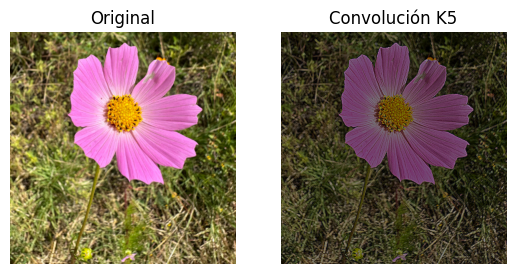
\includegraphics[width=0.7\textwidth]{rsc/k5.png}
        \caption{Resultados con implementación manual (K5)}
\end{figure}
\begin{figure}[H]
        \centering
        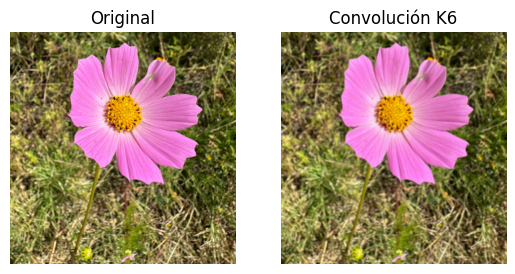
\includegraphics[width=0.7\textwidth]{rsc/k6.png}
        \caption{Resultados con implementación manual (K6)}
\end{figure}

\section{Conclusión}
Se implementaron filtros basados en kernels mediante convolución tanto con OpenCV como de forma manual. Los resultados obtenidos fueron 
consistentes entre ambos métodos, validando la correcta aplicación de la operación de convolución. La manipulación de los valores del 
kernel permitió observar efectos variados en la imagen, como detección de bordes, realce y suavizado. 
Con esta prueba podemos observar además del comportamiento de la librería OpenCV (Implementación rápida y sencilla), la importancia 
de los parámetros en la convolución y cómo afectan el resultado final, asi como la vista paso a paso de la operacion al implementarla manualmente.



%\begin{thebibliography}{00}
%\bibliography{references}
%\end{thebibliography}


\end{document}


